\documentclass[11pt]{article}
\usepackage[margin=0.9in]{geometry}
\usepackage{amsmath,amssymb,bm}
\usepackage{fontspec}
\setmonofont{DejaVu Sans Mono}[Scale=0.78]
\usepackage{graphicx,booktabs,float,fancyvrb,xcolor,hyperref}
\hypersetup{colorlinks=true,linkcolor=blue,urlcolor=blue}
\setlength{\parskip}{4pt}\setlength{\parindent}{0pt}
\newcommand{\x}{{\mathbf{x}}}
\DeclareMathOperator*{\argmin}{arg\,min}\DeclareMathOperator*{\argmax}{arg\,max}

\title{EECE5644 Fall 2026 -- Assignment 3}
\author{David Abu}
\date{}
\begin{document}
\maketitle

\noindent All experiments were implemented in Python 3 (NumPy, SciPy, scikit-learn, joblib, Matplotlib) with fixed random seeds, so every number below is reproducible from the code in the Appendix.

%=====================================================================
\section*{Question 1: MLP approximation of class posteriors}

\subsection*{Data distribution}
There are $C=4$ classes with uniform priors $P(L=c)=1/4$ and Gaussian class-conditional pdfs $p(\x|L=c)=\mathcal N(\x;\bm\mu_c,\Sigma_c)$, $\x\in\mathbb R^3$. The means sit on the vertices of a regular tetrahedron scaled by $s=0.85$:
\[
\bm\mu_1=s[1,1,1]^T,\quad \bm\mu_2=s[1,-1,-1]^T,\quad \bm\mu_3=s[-1,1,-1]^T,\quad \bm\mu_4=s[-1,-1,1]^T .
\]
Each covariance is $\Sigma_c=R_c\,\mathrm{diag}(\bm\lambda_c)\,R_c^T$ with a different rotation $R_c$ and eigenvalues
$\bm\lambda_1=(1.0,0.6,0.3)$, $\bm\lambda_2=(0.8,0.8,0.4)$, $\bm\lambda_3=(1.2,0.5,0.5)$, $\bm\lambda_4=(0.7,0.6,0.9)$, so the classes have different shapes and orientations and the optimal decision boundaries are quadratic. The rotation angles are listed in \texttt{q1.py}. The scale $s$ was tuned by Monte Carlo (200{,}000 samples per candidate): $s=0.8,0.9,1.0$ gave Bayes errors of $17.2\%$, $12.8\%$ and $9.1\%$, so $s=0.85$ places the optimal error near the middle of the required 10--20\% range.

Training sets with $N\in\{100,500,1000,5000,10000\}$ samples and a test set with 100{,}000 samples were drawn independently. The test set was used only for final performance evaluation. Its class counts are <<TEST_COUNTS>>.

\begin{figure}[H]\centering
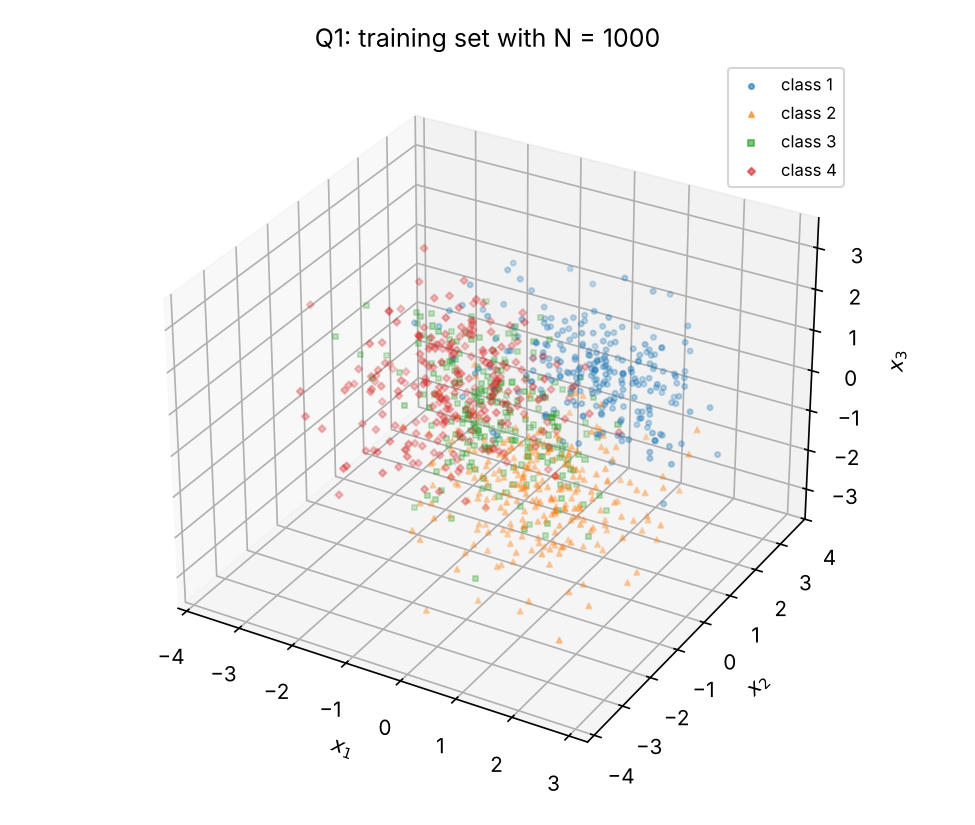
\includegraphics[width=0.55\linewidth]{figs/q1_data.png}
\caption{The $N=1000$ training set.}
\end{figure}

\subsection*{Theoretically optimal classifier}
With 0--1 loss, the minimum-expected-risk rule is the MAP rule
\[
D(\x)=\argmax_{c}\;P(L=c|\x)=\argmax_c\;\Big[\ln\mathcal N(\x;\bm\mu_c,\Sigma_c)+\ln P(L=c)\Big],
\]
which, with uniform priors, reduces to choosing the largest class-conditional log-likelihood. Applied to the test set with the true pdfs, it gives
\[
\boxed{\hat P_{\text{opt}}(\text{error})=<<PE_OPT>>}
\]
This is the aspirational performance level for the MLPs. Its confusion counts are:
<<CONF_TABLE>>

\subsection*{MLP model}
Each model is a two-layer MLP: $P$ hidden perceptrons with the smooth-ReLU (softplus) activation $\phi(a)=\ln(1+e^{a})$, followed by a softmax output layer:
\[
\mathbf h=\phi\big(W_1\tilde\x+\mathbf b_1\big)\in\mathbb R^P,\qquad
\hat P(L=c|\x)=y_c(\x)=\frac{\exp\big(\mathbf w_{2,c}^T\mathbf h+b_{2,c}\big)}{\sum_{k=1}^C\exp\big(\mathbf w_{2,k}^T\mathbf h+b_{2,k}\big)} .
\]
Here $\tilde\x$ is $\x$ standardized with the mean and standard deviation of the data the model is trained on, so validation and test data are never used for standardization. The model has $P(d+1)+C(P+1)=8P+4$ parameters $\bm\theta$. The softmax guarantees $y_c>0$ and $\sum_cy_c=1$.

\textbf{Maximum-likelihood training.} For iid training data $\{(\x_n,l_n)\}_{n=1}^N$ with one-hot labels $t_{nc}$, the likelihood of the labels under the model is $\prod_n\prod_c y_c(\x_n)^{t_{nc}}$. So the ML estimate minimizes the average cross-entropy
\[
\hat{\bm\theta}_{ML}=\argmin_{\bm\theta}\;-\frac1N\sum_{n=1}^N\sum_{c=1}^C t_{nc}\ln y_c(\x_n;\bm\theta).
\]
No regularization term is added, so this is pure ML as the question specifies. The objective is minimized with full-batch L-BFGS (\texttt{scipy.optimize.minimize}, method \texttt{L-BFGS-B}). The gradient is computed analytically by backpropagation: $\partial/\partial\mathbf a_2=(\mathbf y-\mathbf t)/N$ at the softmax, then back through $W_2$ and the softplus derivative $\phi'(a)=\sigma(a)=1/(1+e^{-a})$. Weights are initialized randomly (Glorot-style normal draws), with a fresh draw for every restart.

\textbf{Local optima.} The cross-entropy of an MLP is non-convex. Every training call therefore runs several independent random initializations and keeps the solution with the \emph{highest training log-likelihood} (lowest average cross-entropy). The final models use 10 restarts (up to 3000 L-BFGS iterations each). The cross-validation fits use 2 restarts (up to 1000 iterations each) to keep the computation manageable.

\textbf{Classification.} Treating $y_c(\x)$ as the class posterior, the MAP rule is $D(\x)=\argmax_c y_c(\x)$.

\subsection*{Model-order selection by 10-fold cross-validation}
For each training set, the candidate hidden-layer sizes were $P\in\{<<P_GRID>>\}$. The training set was shuffled and split into 10 disjoint folds (\texttt{sklearn.model\_selection.KFold}). For each $P$ and each fold, an MLP was trained by ML on the other 9 folds and used to classify the held-out fold. The CV objective is the total number of validation errors summed over the 10 folds, divided by $N$: an estimate of P(error) in which every sample is classified exactly once by a model that did not see it. The selected $P$ minimizes this estimate, with ties broken toward the smaller network. The 100 fits per training set (10 values of $P$ $\times$ 10 folds) ran in parallel with \texttt{joblib}.

\begin{figure}[H]\centering
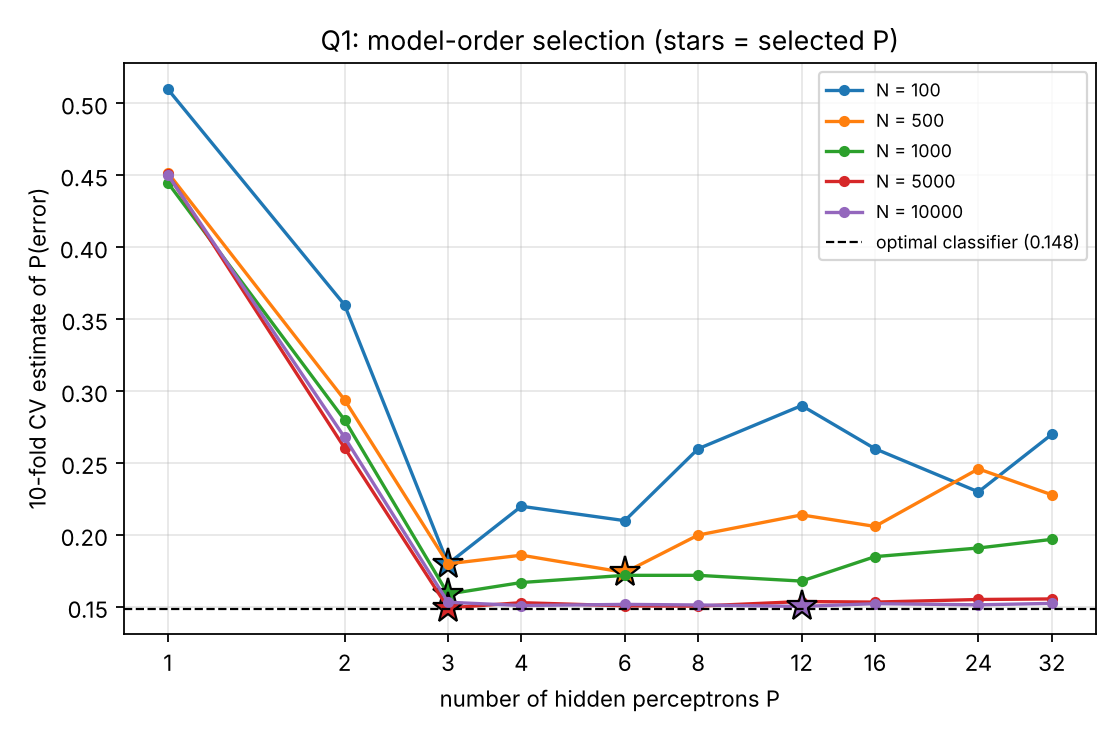
\includegraphics[width=0.78\linewidth]{figs/q1_cv.png}
\caption{10-fold CV estimate of P(error) versus $P$ for each training set. Stars mark the selected $P$; the dashed line is the optimal classifier's test error.}
\end{figure}

<<CV_TABLE>>

\subsection*{Final training and test-set performance}
For each training set, an MLP with the selected $P$ was retrained by ML on the \emph{entire} training set with 10 random restarts, keeping the highest-likelihood solution. Each final model then classified the 100{,}000 test samples with the MAP rule.

<<FINAL_TABLE>>

\begin{figure}[H]\centering
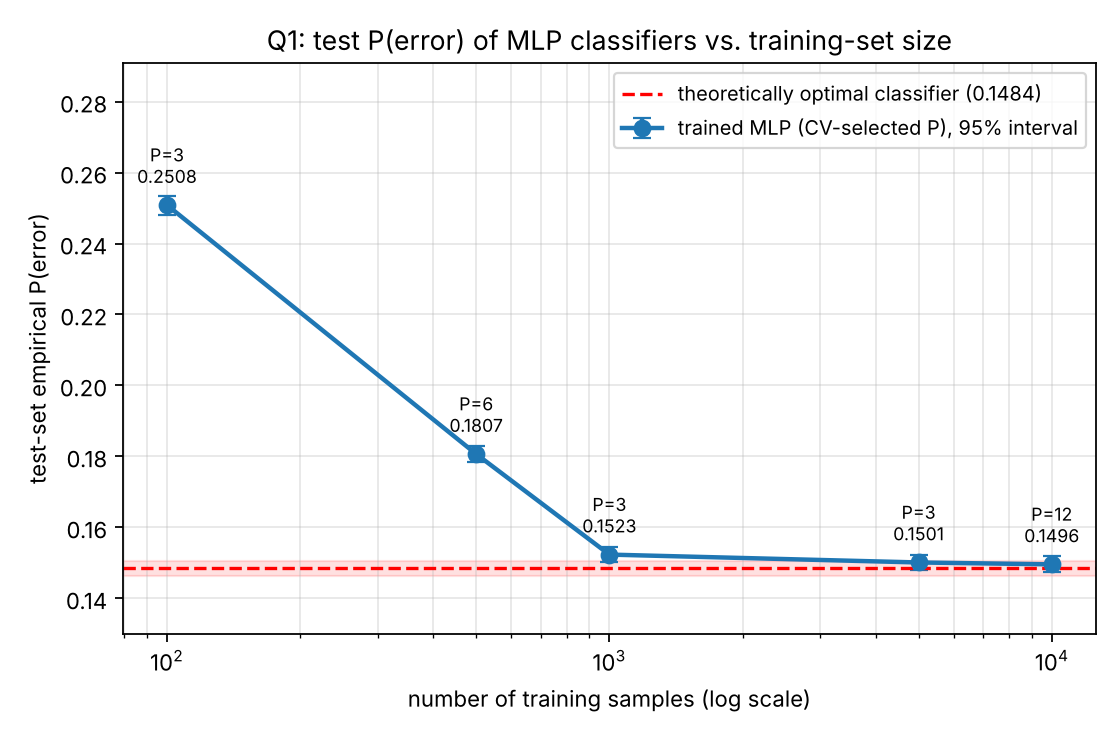
\includegraphics[width=0.8\linewidth]{figs/q1_test_perror.png}
\caption{Test-set empirical P(error) of each trained MLP versus the number of training samples (semilog-$x$), with 95\% Wilson binomial intervals. The red dashed line and band are the theoretically optimal classifier and its interval. The intervals reflect test-set sampling only, not variability over training sets or initializations; all classifiers share the same test set.}
\end{figure}

\begin{figure}[H]\centering
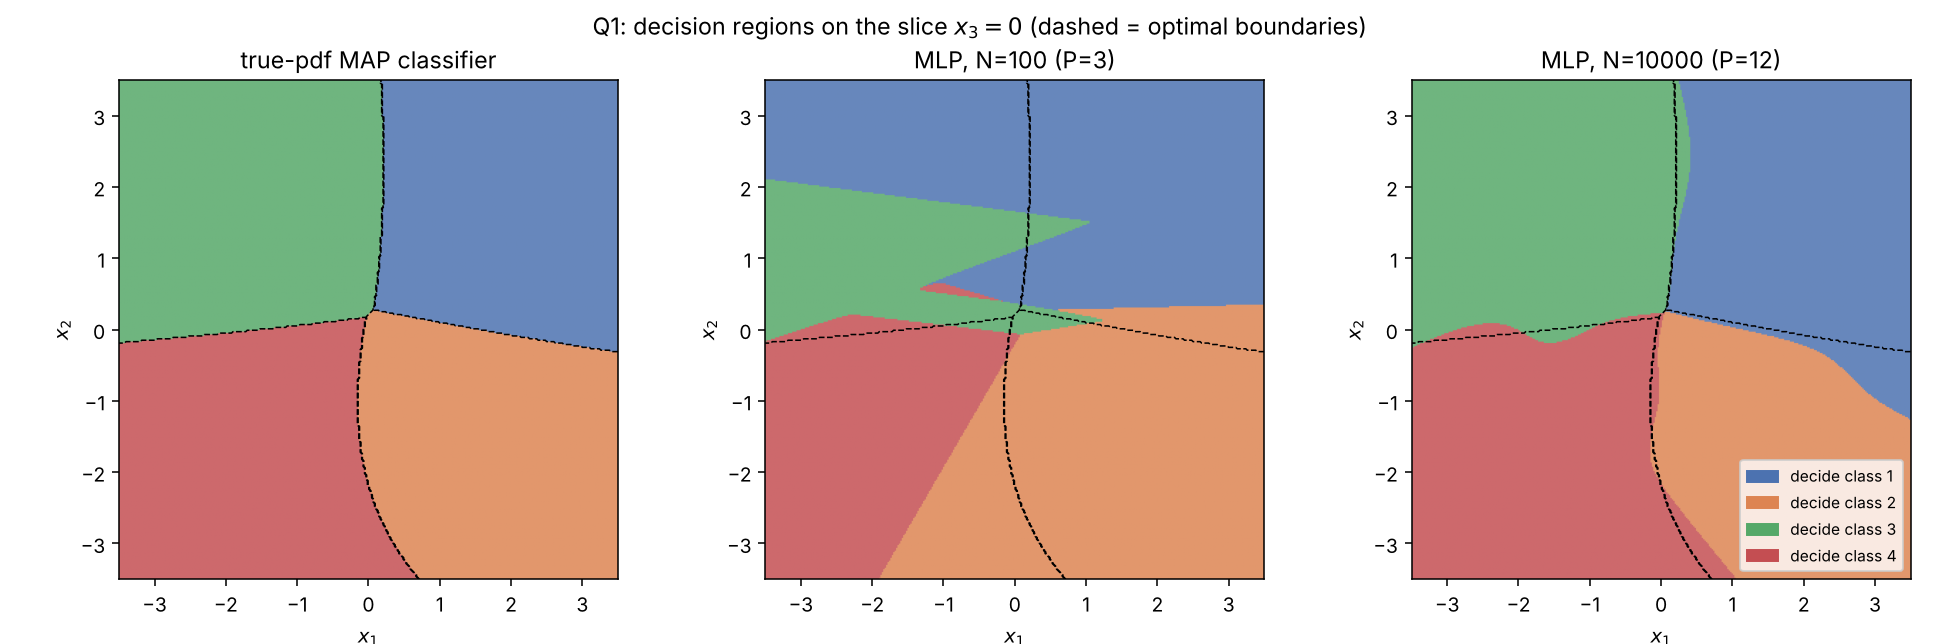
\includegraphics[width=\linewidth]{figs/q1_decision_slice.png}
\caption{Decision regions on the plane $x_3=0$, a slice of the 3-D classifiers, for the true-pdf MAP rule, the $N=100$ MLP and the $N=10000$ MLP. Dashed lines are the optimal boundaries. The $N=10000$ MLP reproduces the curved optimal boundaries closely, while the $N=100$ model's regions are visibly distorted.}
\end{figure}

<<CONF_MLP_TABLE>>

\subsection*{Discussion}
<<Q1_DISCUSSION>>

\subsection*{How the software was verified}
\begin{itemize}
\item \textbf{Gradient.} The MLP and its backpropagation were written directly in NumPy, so the gradient was checked against a central finite-difference approximation (\texttt{scipy.optimize.approx\_fprime}) at a random parameter vector. The relative error was <<GRAD_ERR>>, confirming that L-BFGS receives the exact gradient of the cross-entropy it minimizes.
\item \textbf{Outputs.} The softmax outputs were checked to be positive and to sum to 1 for every sample. The log-softmax is computed by subtracting the row maximum, and softplus as \texttt{logaddexp(0,a)}, so neither overflows for large activations.
\item \textbf{Objective.} The loss is exactly the average negative log-likelihood of the one-hot labels under the softmax outputs, i.e.\ the ML criterion. No weight decay or early stopping is applied, and every L-BFGS run starts from a new random initialization.
\item \textbf{Cross-validation.} The code asserts that the 10 validation folds are disjoint from their training folds and together cover every training sample exactly once. Standardization statistics are recomputed inside each training call, so no validation data leak into training.
\item \textbf{Test set.} The 100{,}000-sample test set is used only after model selection and final training, never for choosing $P$ or for stopping.
\item \textbf{Optimizer convergence.} The L-BFGS status of every restart was recorded by re-running the final fits and all cross-validation fits with their original seeds. The script asserts that every error count reproduces exactly. Here ``converged'' means the projected gradient fell below $10^{-7}$ before the iteration cap, a deliberately strict tolerance.
<<CONV_TABLE>>
Non-converged runs stopped at the iteration cap while still making very small improvements. They are kept at their achieved likelihood, never discarded. Non-convergence is rare at $N=100$ (86\% of retained CV fits converged) and common for $N\ge500$ (15--20\%). Unpenalized cross-entropy has very flat directions, along which weights can keep growing to sharpen posteriors that are already nearly right, so the strict gradient tolerance is hard to meet within the budget. The sensitivity check below tests whether this affects the selected sizes. The spread of final training NLL across the 10 restarts (last column) shows how much the restarts mattered.

\textbf{Does non-convergence affect model selection?} Because many CV fits stopped at the 1000-iteration cap, the CV for $N=500$ and $N=1000$ was repeated with a 5$\times$ larger budget of 5000 iterations, using the same seeds and folds (\texttt{q1\_cv\_sensitivity.py}). <<SENS_TEXT>>
<<SENS_TABLE>>
Running longer leaves small networks unchanged and makes large networks slightly \emph{worse} on held-out data: they fit the training folds more closely. The iteration cap therefore acts as mild implicit regularization on oversized networks, but it does not change which $P$ is selected.
\item \textbf{End-to-end.} With 10{,}000 training samples, the MLP's test error comes within <<GAP_10K>> of the true-pdf MAP classifier, as expected of a consistent posterior estimator with enough data and capacity.
\end{itemize}

%=====================================================================
\section*{Question 2: GMM model-order selection with cross-validation}

\subsection*{True GMM}
The true density is $p(\x)=\sum_{k=1}^4\alpha_k\,\mathcal N(\x;\bm\mu_k,\Sigma_k)$, $\x\in\mathbb R^2$, with
\begin{center}
\begin{tabular}{ccccc}\toprule
$k$ & $\alpha_k$ & $\bm\mu_k$ & $\Sigma_k$ & mean eigenvalue of $\Sigma_k$\\\midrule
1 & 0.30 & $[0,\,0]^T$ & $\begin{bmatrix}1.0&0.3\\0.3&0.8\end{bmatrix}$ & <<EIG1>>\\[8pt]
2 & 0.25 & $[1.6,\,0.6]^T$ & $\begin{bmatrix}0.7&-0.2\\-0.2&1.0\end{bmatrix}$ & <<EIG2>>\\[8pt]
3 & 0.25 & $[6,\,4]^T$ & $\begin{bmatrix}1.5&0.6\\0.6&0.9\end{bmatrix}$ & <<EIG3>>\\[8pt]
4 & 0.20 & $[-5,\,5]^T$ & $\begin{bmatrix}0.6&0\\0&1.8\end{bmatrix}$ & <<EIG4>>\\\bottomrule
\end{tabular}
\end{center}
All four components have different weights, means and covariances. Components 1 and 2 overlap strongly: their means are $\|\bm\mu_1-\bm\mu_2\|=<<DIST12>>$ apart, while the sum of their average covariance eigenvalues is $<<EIGSUM>>$, the same order as the question suggests. Together they form a single elongated lump. Components 3 and 4 are well separated from everything else.

\begin{figure}[H]\centering
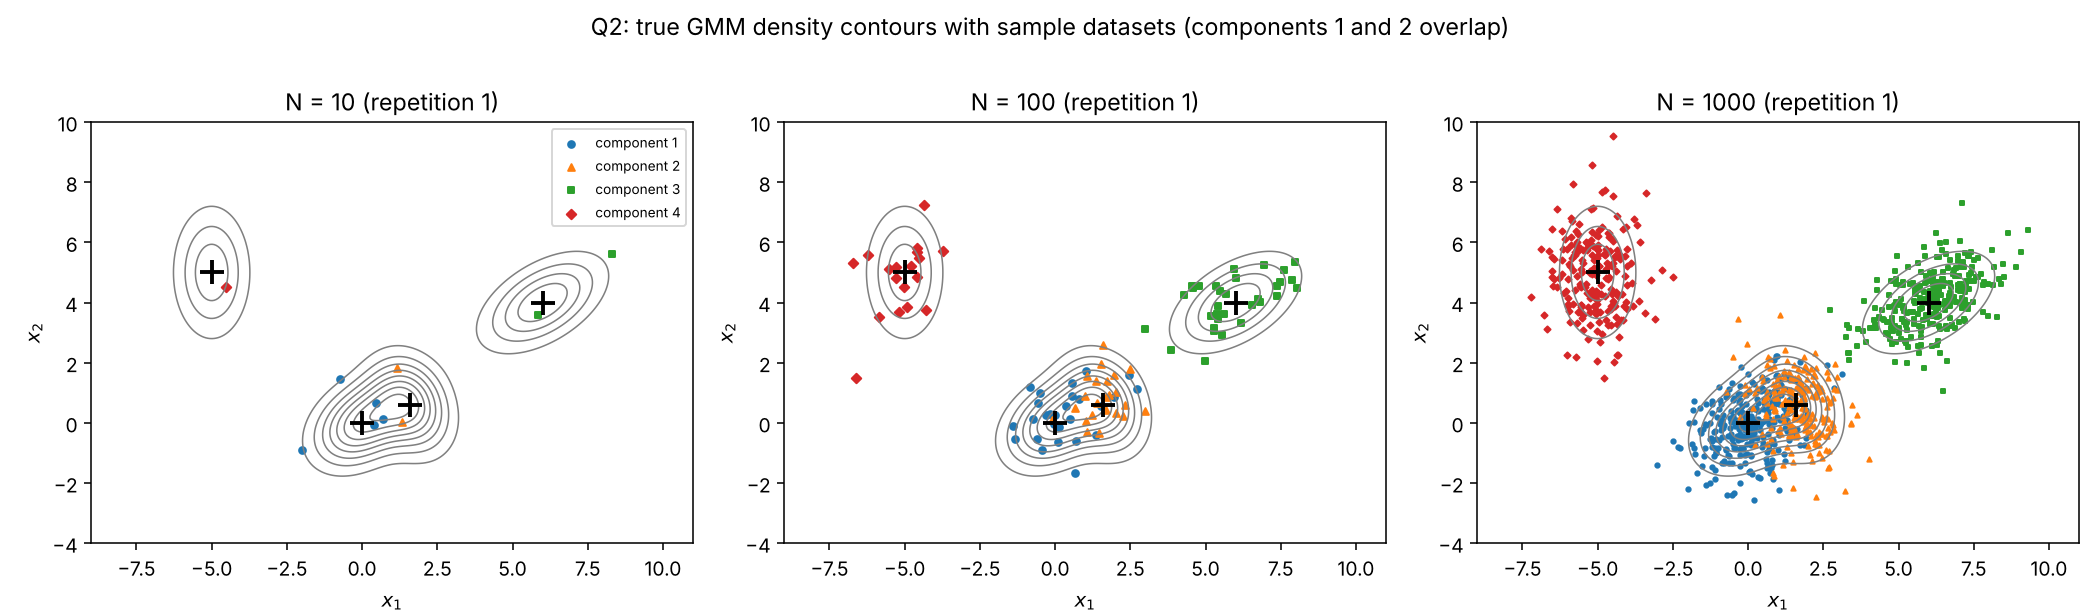
\includegraphics[width=\linewidth]{figs/q2_data.png}
\caption{True GMM density contours with one dataset of each size, colored by the (hidden) generating component.}
\end{figure}

\subsection*{Procedure}
For each repetition $r=1,\dots,R$ with $R=<<R>>$, and each size $N\in\{10,100,1000\}$:
\begin{enumerate}
\item Draw a fresh iid dataset of $N$ samples from the true GMM.
\item Shuffle it and split it into 10 disjoint folds. For $N=10$ each fold holds one sample, so this is leave-one-out.
\item For each candidate order $K=1,\dots,10$ and each fold, fit a $K$-component, full-covariance GMM to the other 9 folds by maximum likelihood with the EM algorithm (scikit-learn's \texttt{GaussianMixture}). Then compute the log-likelihood of the held-out fold under the fitted model, $\sum_{\x\in\text{fold}}\ln\hat p_K(\x)$.
\item Sum the held-out log-likelihoods over the 10 folds; dividing by $N$ gives the average validation log-likelihood $\overline{\ell}_K$. Every sample is scored exactly once by a model that did not see it.
\item Select $\hat K=\argmax_K\overline{\ell}_K$.
\end{enumerate}
The selection rate of order $K$ at size $N$ is the fraction of the $R$ repetitions with $\hat K=K$. Both parameter estimation (EM maximizes training log-likelihood) and validation (held-out log-likelihood) use the log-likelihood of the data, as the question requires.

\textbf{EM settings and why.}
\begin{itemize}
\item \emph{Local optima.} Each EM fit runs 3 k-means++ initializations (\texttt{n\_init=3}) and keeps the highest-likelihood solution, with up to 500 iterations and tolerance $10^{-4}$.
\item \emph{Covariance floor.} The GMM likelihood is unbounded: a component can collapse onto a single training point with covariance $\to0$. To keep the ML problem well posed, $10^{-3}I$ is added to every covariance estimate (\texttt{reg\_covar}). This is negligible compared with the true covariances, whose eigenvalues are 0.5--1.9. A collapsed component still wastes probability mass on held-out points, so CV still penalizes overfitting.
\item \emph{Infeasible orders.} A $K$-component GMM cannot be fitted to fewer than $K$ points. For $N=10$ each training split has 9 samples, so $K=10$ is assigned validation log-likelihood $-\infty$ and can never be selected. This is a real limitation of 10 samples, not a software artifact.
\end{itemize}

\subsection*{Results}
<<RATE_TABLE>>

\begin{figure}[H]\centering
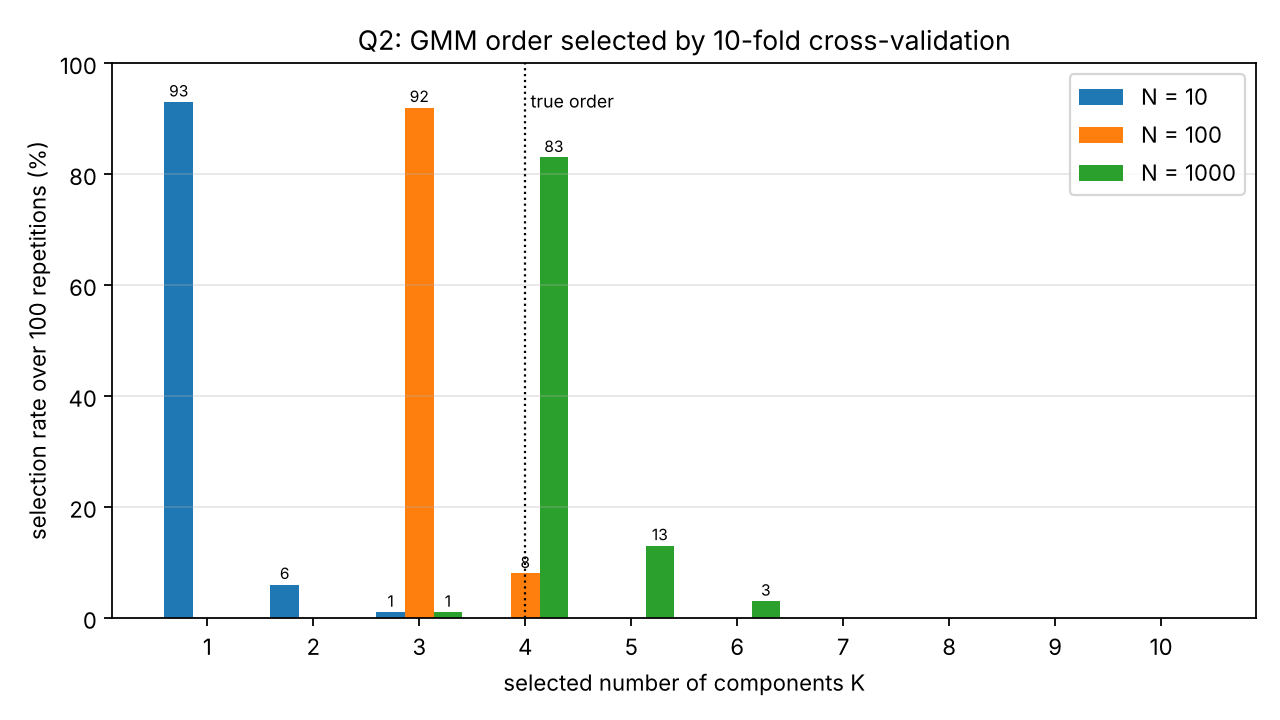
\includegraphics[width=0.85\linewidth]{figs/q2_selection_rates.png}
\caption{Selection rate of each GMM order over <<R>> repetitions, for each dataset size.}
\end{figure}

\begin{figure}[H]\centering
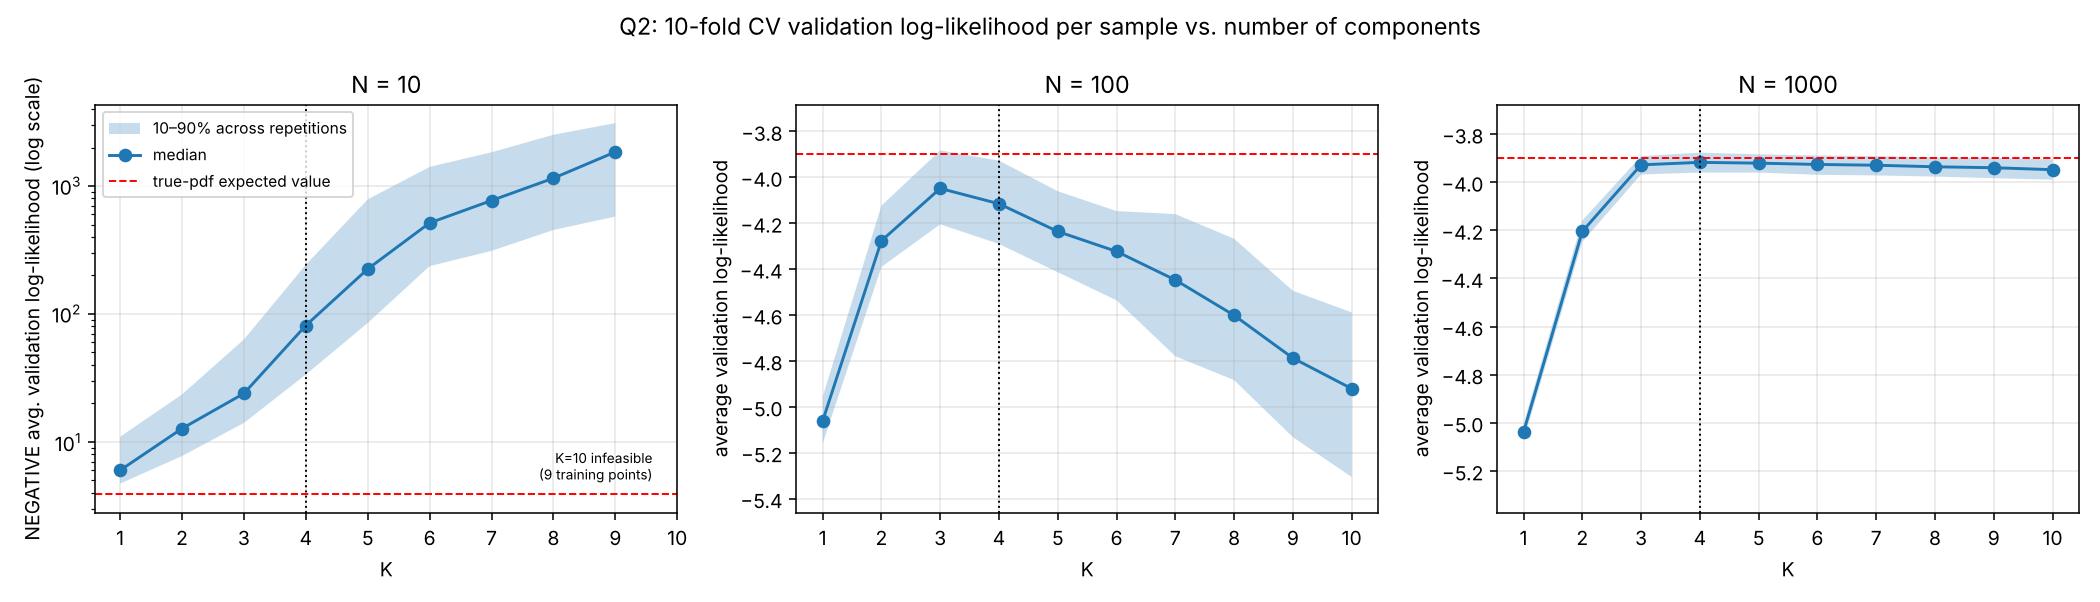
\includegraphics[width=\linewidth]{figs/q2_cv_curves.png}
\caption{Average validation log-likelihood per sample versus $K$: median and 10--90\% band across repetitions. The red line is $E[\ln p_{\text{true}}(\x)]\approx<<LL_TRUE>>$, estimated with 200{,}000 samples; it is the best value any model can achieve in expectation. For $N=10$ the $y$-axis is clipped because large-$K$ fits collapse onto single points and give very negative held-out scores.}
\end{figure}

\subsection*{Discussion}
<<Q2_DISCUSSION>>

%=====================================================================
\section*{Acknowledgement of resources and AI use}
\textbf{[EDIT BEFORE SUBMITTING: make this statement accurately describe how you used these tools, then delete this line.]}
I used Claude (Anthropic, model Claude Opus 5.5, via claude.ai, November 2026) as a coding and writing assistant for this assignment. It helped design the data distributions, write the Python implementations in the Appendix, run the experiments, produce the figures, and draft and typeset this report. I reviewed the procedures and results. Libraries used: NumPy, SciPy (\texttt{scipy.optimize.minimize}, \texttt{scipy.stats.multivariate\_normal}), scikit-learn (\texttt{KFold}, \texttt{GaussianMixture}), joblib, and Matplotlib.

%=====================================================================
\newpage
\section*{Appendix: Code}
\subsection*{mlp.py}
\VerbatimInput[fontsize=\scriptsize,frame=single]{mlp.py}
\subsection*{q1.py}
\VerbatimInput[fontsize=\scriptsize,frame=single]{q1.py}
\subsection*{q1\_diagnostics.py}
\VerbatimInput[fontsize=\scriptsize,frame=single]{q1_diagnostics.py}
\subsection*{q1\_cv\_sensitivity.py}
\VerbatimInput[fontsize=\scriptsize,frame=single]{q1_cv_sensitivity.py}
\subsection*{q2.py}
\VerbatimInput[fontsize=\scriptsize,frame=single]{q2.py}
\end{document}
